\documentclass[a4paper,UTF8]{article}
\usepackage{ctex}
\usepackage[margin=1.25in]{geometry}
\usepackage{color}
\usepackage{graphicx}
\usepackage{amssymb}
\usepackage{amsmath}
\usepackage{amsthm}
\usepackage{soul, color, xcolor}
\usepackage{bm}
\usepackage{tcolorbox}
\usepackage{hyperref}
\numberwithin{equation}{section}
%\usepackage[thmmarks, amsmath, thref]{ntheorem}
\theoremstyle{definition}
\newtheorem*{solution}{Solution}
\newtheorem*{prove}{Proof}
\usepackage{multirow}
\usepackage{diagbox}
\usepackage{float}

\usepackage{caption}
\usepackage{subcaption}

\def \X {\mathbf{X}}
\def \W {\mathbf{W}}
\def \A {\mathbf{A}}
\def \K {\mathbf{K}}
\def \B {\mathbf{B}}
\def \C {\mathbf{C}}
\def \Q {\mathbf{Q}}
\def \S {\mathbf{S}}
\def \P {\mathbf{P}}
\def \Diag {\textbf{$\Lambda$}}
\def \w {\hat{\boldsymbol{w}}}
\def \y {\boldsymbol{y}}
\def \x {\boldsymbol{x}}
\def \z {\mathbf{z}}
\def \b {\mathbf{b}}
\def \by {\Bar{y}}
\def \H {\mathbf{H}}
\def \I {\mathbf{I}}
\setlength{\parindent}{0pt}

\newcommand{\vct}[1]{\boldsymbol{#1}} % vector
\newcommand{\vw}{\vct{w}}
\newcommand{\vx}{\vct{x}}
\newcommand{\vy}{\vct{y}}
\newcommand{\vzero}{\vct{0}}
\newcommand{\ones}{\vct{1}}

\newcommand{\mat}[1]{\boldsymbol{#1}} % matrix
\newcommand{\mI}{\mat{I}}
\newcommand{\mQ}{\mat{Q}}
\newcommand{\mX}{\mat{X}}

\usepackage{listings}
\def\codecommentcolor{\color{cyan}} % 定义代码中注释的颜色
\newcommand*{\codecomment}[1]{\hfill\makebox[0.38\textwidth][l]{\codecommentcolor{}{\# #1}}} % 代码行末注释的指令, 用于以绝对位置对齐行末注释
\lstset{language=Python}
\lstset{
	breaklines,
	basicstyle=\ttfamily\footnotesize,
	backgroundcolor=\color[rgb]{0.95,0.95,0.95},
	commentstyle=\codecommentcolor{},
	tabsize=4,numbers=left,
	numberstyle=\tiny,
	frame=single,
	numberstyle=\tiny,
	numbersep=5pt, 
	tabsize=2,
	extendedchars=false,
	breaklines=true,
	keywordstyle=\color{red},
	stringstyle=\color{pink}\ttfamily,
	showspaces=false,
	showtabs=false,
	xleftmargin=17pt,
	framexleftmargin=17pt,
	framexrightmargin=5pt,
	framexbottommargin=4pt,
	showstringspaces=false,
	escapechar=\&
}
\renewcommand{\lstlistingname}{CODE}
\lstloadlanguages{% Check Documentation for further languages ...
	%[Visual]Basic
	%Pascal
	%C
	Python
	%XML
	%HTML
	%Java
}
%--
%\begin{equation}
%    \begin{aligned}

%    \end{aligned}
%\end{equation}
%--
\begin{document}
\title{机器学习导论\ 习题四}
\author{221300079, 王俊童, \href{mailto:221300079@smail.nju.edu.cn}{221300079@smail.nju.edu.cn}}
\maketitle
\section*{作业提交注意事项}
\begin{tcolorbox}
    \begin{enumerate}
        \item[1.] 作业所需的LaTeX及Python环境配置要求请参考: \href{https://www.lamda.nju.edu.cn/ML2024Spring/supplemantary/environment.pdf}{[Link]};
        \item[2.] 请在LaTeX模板中第一页填写个人的学号、姓名、邮箱;
        \item[3.] 本次作业需提交的文件为:
        \begin{enumerate}
            \item [(a)] 作答后的LaTeX代码 --- \texttt{HW4.tex};
            \item [(b)] 由(a)编译得到的PDF文件 --- \texttt{HW4.pdf};
            \item [(c)] 题目2.(2)的求解代码文件 --- \texttt{svm\_qp\_dual.py}
            \item [(d)] 题目3的求解代码文件 --- \texttt{svm\_kernel\_solution.py}
        \end{enumerate}
        其他文件 (如其他代码、图片等) 无需提交. 请将以上文件{\color{red}\textbf{打包为~\texttt{学号\hspace{0em}\_\hspace{0em}姓名.zip}}} (例如 \texttt{221300001\hspace{0em}\_\hspace{0em}张三.zip}) 后提交;
        \item[3.] 若多次提交作业, 则在命名~.zip 文件时加上版本号, 例如 \texttt{221300001\_\hspace{0em}张三\hspace{0em}\_v1.zip}” (批改时以版本号最高的文件为准);
        \item[4.] 本次作业提交截止时间为 {\color{red}\textbf{ 5 月 28 日 23:59:59}}. 未按照要求提交作业, 提交作业格式不正确, {\color{red}\textbf{作业命名不规范}}, 将会被扣除部分作业分数; 除特殊原因 (如因病缓交, 需出示医院假条) 逾期未交作业, 本次作业记 0 分; {\color{red}\textbf{如发现抄袭, 抄袭和被抄袭双方成绩全部取消}};
        \item[5.] 学习过程中, 允许参考 ChatGPT 等生成式语言模型的生成结果, 但必须在可信的信息源处核实信息的真实性; {\color{red}\textbf{不允许直接使用模型的生成结果作为作业的回答内容}}, 否则将视为作业非本人完成并取消成绩;
        \item[6.] 本次作业提交地址为 \href{https://box.nju.edu.cn/u/d/9c31a6ce4970487183a9/}{[Link]}, 请大家预留时间提前上交, 以防在临近截止日期时, 因网络等原因无法按时提交作业.
    \end{enumerate}
\end{tcolorbox}
\newpage

\section{[35pts] Soft Margin}
考虑软间隔SVM问题, 其原问题形式如下:
\begin{equation}
    \begin{aligned}
        \min _{\vw, b, \xi_{i}} \quad & \frac{1}{2}\|\vw\|_{2}^{2}+C \sum_{i=1}^{m} \xi^p_{i} \\
        \text { s.t. } \quad & y_{i}\left(\vw^{\top} \vx_{i}+b\right) \geq 1- \xi_{i} \\
        & \xi_{i} \geq 0, i \in [m] .
    \end{aligned}
    \label{soft-margin}
\end{equation}
其中, 松弛变量$\bm{\xi} = \{\xi_i\}_{i=1}^m, \xi_i > 0$表示样本$\vx_i$对应的间隔约束不满足的程度, 在优化问题中加入惩罚$C\sum_{i=1}^m \xi^p_i, C>0, p\ge 1$使得不满足约束的程度尽量小($\xi_i\rightarrow 0$). 课本式(6.35)即为$p=1$时对应的情况, 此时, 所有违反约束的样本都会受到相同比例的惩罚,而不考虑它们违反约束的程度. 这可能导致模型对较大偏差的样本不够敏感,不足以强调更严重的违规情况. 下面将考虑一些该问题的变式:
\begin{enumerate}
    \item[(1)] \textbf{[2+7pts]} 我们首先考虑$p=2$的情况, 它对于违反约束程度较大的样本提供了更大的惩罚. 
    \begin{enumerate}
        \item[(a)] 如课本式(6.34)-(6.35)所述, $p=1$的情况对应了hinge损失$\ell_{hinge} :x \to \max(0, 1-x)$. 请直接写出$p=2$的情况下对应的损失函数. 
        \item[(b)] 请推导$p=2$情况下软间隔SVM的对偶问题. 
    \end{enumerate}
    \item[(2)] \textbf{[14pts]} $p=1$的情况下, 相当于对向量$\bm{\xi}$使用$\mathrm{L}_1$范数惩罚: $\lVert \bm{\xi} \rVert_1 = \sum_{i}  |\xi_i|$. 现在, 我们考虑使用$\mathrm{L}_\infty$范数惩罚: $\lVert \bm{\xi} \rVert_\infty = \max_i  \xi_i $, 这会使得模型着重控制最大的违背约束的程度,从而促使模型在最坏情况下的表现尽可能好. 请推导使用$\mathrm{L}_\infty$范数惩罚的原问题和对偶问题.
    \item[(3)] \textbf{[4+8pts]} 在\eqref{soft-margin}中, 正例和负例在目标函数中分类错误的“惩罚”是相同的. 然而在实际场景中, 很多时候正例和负例错分的“惩罚”代价是不同的 (参考教材2.3.4节). 比如考虑癌症诊断问题, 将一个确实患有癌症的人误分类为健康人, 以及将健康人误分类为患有癌症, 产生的错误影响以及代价不应该认为是等同的. 所以我们考虑对负例分类错误的样本施加$k>0$倍于正例中被分错的样本的“惩罚”. 
    \begin{enumerate}
        \item[(a)] 令\eqref{soft-margin}中$p=1$, 并令所有正例样本的集合为 $D_{+}$, 负例样本的集合为 $D_{-}$. 请给出相应的SVM优化问题.
        \item[(b)] 请给出相应的对偶问题.
    \end{enumerate}
\end{enumerate}

\begin{solution}
现在给出这个题的解答:\\
(1).p = 2\\
(a).因为此时总的间隔是4,我们可以得到:\\
\[  r = \frac{4}{\|\vw\|_{2}^{2}}  \]
所以对于需要优化的函数:\\
\[  \min _{\vw, b, \xi_{i}} \quad  \frac{1}{2}\|\vw\|_{2}^{2}+C \sum_{i=1}^{m} \xi^2_{i}\]
其中$\xi$是松弛变量。通过这个式子可以推导损失函数:
\[  \ell_{hinge} :x \to \max(0, (1 - y_i (\vw^{\top}x_i + b)))^2\]
(b).下面给出对偶问题的具体推导,使用拉格朗日乘子法,首先可以得到原问题如下:\\
\begin{equation}
    \begin{aligned}
        \min _{\vw, b, \xi_{i}} \quad & \frac{1}{2}\|\vw\|_{2}^{2}+C \sum_{i=1}^{m} \xi^2_{i} \\
        \text { s.t. } \quad & y_{i}\left(\vw^{\top} \vx_{i}+b\right) \geq 1- \xi_{i} \\
        & \xi_{i} \geq 0, i \in [m] .
    \end{aligned}
\end{equation}
所以可以得到拉格朗日函数如下:\\
\[  L(\vw, b, \xi, \alpha, \beta) = \frac{1}{2}\|\vw\|_{2}^{2} + C \sum_{i=1}^{m} \xi^2_{i} - \sum_{i=1}^{m} \alpha_i( y_{i}(\vw^{\top} \vx_{i}+b) - 1 + \xi_{i}) - \sum_{i=1}^{m} \beta_i \xi_{i}    \]
对w,b,$\xi$分别求偏导:\\
\[  \frac{\partial L}{\partial \vw} = w  - \sum_{i=1}^{m}\alpha_i y_i x_i = 0\]
\[  \frac{\partial L}{\partial b} =  \sum_{i=1}^{m}\alpha_i y_i  = 0\]
\[  \frac{\partial L}{\partial \xi} = 2C\xi_i - \mu_i - \alpha_i = 0\]
带入原式子化简可以得到对偶问题:\\
\begin{equation}
    \begin{aligned}
        \min _{\alpha} \quad & \sum_{i=1}^{m}\alpha_i - \sum_{i=1}^{m}\frac{(\alpha_i + \beta_i)^2}{4C}\\
        \text { s.t. } \quad &  \sum_{i=1}^{m}\alpha_i y_i  = 0\\
        & 0 \leq \alpha_i \leq 2C, i \in [m] .
    \end{aligned}
\end{equation}

(2)若损失函数换成$L_{\infty}$范数作为惩罚,令$||\xi||_{\infty} = max|\xi_i|$,我们可以得到原问题形式:\\
\begin{equation}
    \begin{aligned}
        \min _{\vw, b, \xi_{i}} \quad & \frac{1}{2}\|\vw\|_{2}^{2}+C ||\xi||_{\infty}\\
        \text { s.t. } \quad & y_{i}\left(\vw^{\top} \vx_{i}+b\right) \geq 1- \xi_{i} \\
        & \xi_{i} \geq 0, i \in [m] .
    \end{aligned}
\end{equation}
这个原问题的等价问题等于:\\
\begin{equation}
    \begin{aligned}
        \min _{\vw, b, \eta} \quad & \frac{1}{2}\|\vw\|_{2}^{2}+C \eta\\
        \text { s.t. } \quad & y_{i}\left(\vw^{\top} \vx_{i}+b\right) \geq 1- \xi_{i} \\
        & 0 \leq \xi_i \leq \eta, i \in [m] .
    \end{aligned}
\end{equation}
所以可以得到这个函数的lagrange函数如下形式:\\
\[  L(\vw, b, \xi, \eta, \alpha, r, \beta) = \frac{1}{2}\|\vw\|_{2}^{2} + C \eta - \sum_{i=1}^{m} \alpha_i( y_{i}(\vw^{\top} \vx_{i}+b) - 1 + \xi_{i}) -\sum_{i=1}^{m}r_i \xi_i - \sum_{i=1}^{m} \beta_i (\xi_{i} - \eta)    \]
对w,b,$\xi, \eta$分别求偏导:\\
\[  \frac{\partial L}{\partial \vw} = w  - \sum_{i=1}^{m}\alpha_i y_i x_i = 0\]
\[  \frac{\partial L}{\partial b} =  \sum_{i=1}^{m}\alpha_i y_i  = 0\]
\[  \frac{\partial L}{\partial \xi} = \beta_i - \alpha_i - r_i = 0\]
\[  \frac{\partial L}{\partial \eta} = C  - \sum_{i=1}^{m}\beta_i = 0\]
带入原问题可以得到这个原问题的对偶问题如下所示:\\
\begin{equation}
    \begin{aligned}
        \min _{\alpha} \quad & \sum_{i=1}^{m}\alpha_i - \frac{1}{2}\sum_{i=1}^{m}\sum_{j=1}^{m}\alpha_i \alpha_j y_i y_j x_i^{\top} x_j  \\
        \text { s.t. } \quad &  \sum_{i=1}^{m}\alpha_i y_i  = 0\\\
        & \sum_{i=1}^{m}\alpha_i \leq C \\
        & 0 \leq \alpha_i, i \in [m] .
    \end{aligned}
\end{equation}

(3)对于这个问题,我们假设分类的正确样本和错误样本有数量如下:$D_{+}$ = n, $D_{-}$ = m.同时我们引入不同的惩罚系数$C_{+},C_{-}$,且根据题意具有以下关系$C_{-} = kC_{+}$.\\
(a).所以根据上面所示,这个问题的原问题可以表达如下:
\begin{equation}
    \begin{aligned}
        \min _{\vw, b, \xi_{i}^{+}, \xi_{j}^{-}} \quad & \frac{1}{2}\|\vw\|_{2}^{2}+ C_{+}\sum_{i}^{n}\xi_i^{+} + C_{-}\sum_{j}^{m}\xi_i^{-} \\
        \text { s.t. } \quad & y_{i}\left(\vw^{\top} \vx_{i}+b\right) \geq 1- \xi_{i}^{+} \\
        & y_{j}\left(\vw^{\top} \vx_{j}+b\right) \geq 1- \xi_{j}^{-} \\
        & \xi_{i}^{+} \geq 0, i \in [n] .\\
        & \xi_{j}^{-} \geq 0, j \in [m] .\\
        & C_{-} = kC_{+}\\
    \end{aligned}
\end{equation}
(b).所以可以根据原问题得到这个问题的lagrange函数如下所示:\\
\[  L(\vw, b, \xi_{i}^{+}, \xi_{j}^{-}, \alpha_1, \alpha_2 , \beta_1, \beta_2) = \frac{1}{2}\|\vw\|_{2}^{2} + C_{+} \sum_{i=1}^{n} \xi^{+}_{i}  + C_{-} \sum_{j=1}^{m} \xi^{-}_{j} - \sum_{i=1}^{n} \alpha_{1i}( y_{i}(\vw^{\top} \vx_{i}+b) - 1 + \xi_{i}^{+}) \]
\[- \sum_{j=1}^{m} \alpha_{2j}( y_{j}(\vw^{\top} \vx_{j}+b) - 1 + \xi_{j}^{-})- \sum_{i=1}^{n} \beta_{1i} \xi_{i}^{+} - \sum_{j=1}^{m} \beta_{2j} \xi_{j}^{-}   \]
对w,b,$\xi^{+},\xi^{-}$分别求偏导:\\
\[  \frac{\partial L}{\partial \vw} = \vw  -\sum_{i=1}^{n}\alpha_{1i}y_ix_i -\sum_{j=1}^{m}\alpha_{2j}y_jx_j = 0      \]
\[  \frac{\partial L}{\partial b} = \sum_{i=1}^{n}\alpha_{1i}y_i + \sum_{j=1}^{m}\alpha_{2j} y_j = 0\]
\[  \frac{\partial L}{\partial \xi^{+}} = C_{+} - \alpha_{1i} - \beta_{1i} = 0\]
\[  \frac{\partial L}{\partial \xi^{-}} = C_{-} - \alpha_{2j} - \beta_{2j} = 0\]
所以把这个偏导带入原问题可以得到如下的对偶问题:\\
\begin{equation}
    \begin{aligned}
        \min _{\alpha_{1i},\alpha_{2j}} \quad & \sum_{i=1}^{n}\alpha_{1i} + \sum_{j=1}^{m}\alpha_{2j}  - \frac{1}{2}\sum_{i=1}^{n}\sum_{i=1}^{n}\alpha_i \alpha_j y_i y_j x_i^{\top} x_j - \frac{1}{2}\sum_{j=1}^{m}\sum_{j=1}^{m}\alpha_j \alpha_j y_j y_j x_j^{\top} x_j   \\
        & -\sum_{i=1}^{n}\sum_{j=1}^{m}\alpha_i \alpha_j y_i y_j x_i^{\top} x_j\\
        \text { s.t. } \quad &  \sum_{i=1}^{n}\alpha_{1i}y_i + \sum_{j=1}^{m}\alpha_{2j} y_j = 0\\\
        & 0 \leq \alpha_{1i} \leq C_{+}, i \in [n].\\
        & 0 \leq \alpha_{2j} \leq C_{-}, j \in [m].\\
        & C_{-} = kC_{+}\\
    \end{aligned}
\end{equation}


\end{solution}
\newpage

\section{[20pts] Primal and Dual Problem}
给定一个包含$m$个样本的数据集$D=\{(\vx_i, y_i)\}_{i=1}^{m}$, 其中每个样本的特征维度为$d$, 即$\vx_i \in \mathbb{R}^d$. 软间隔SVM的原问题和对偶问题可以表示为: 
\vspace{8pt}

\begin{minipage}{0.5\textwidth}
原问题:
$$
\begin{aligned}
\min_{\vw, b, \xi} \quad & \frac{1}{2} \vw^{\top} \vw+C \sum_{i=1}^{n} \xi_{i} \\
\text {s.t.}\quad & y_{i}\left(\vw^{\top} \vx_{i}+b\right) \geq 1-\xi_{i}, \forall i \in [m]\\
\quad &\xi_{i} \geq 0, \forall i \in [m]
\end{aligned}
$$
\end{minipage}
\begin{minipage}{0.5\textwidth}
对偶问题:
$$
\begin{aligned}
\min_{\bm{\alpha}}\quad &  \frac{1}{2} \bm{\alpha}^{\top} \mat{Q} \bm{\alpha}-\ones_m^{\top} \bm{\alpha} \\
\text {s.t.}\quad &  \vy^{\top} \bm{\alpha}=0 \\
\quad & 0 \leq \alpha_{i} \leq C, \forall i \in [m]
\end{aligned}
$$
\end{minipage}

\vspace{5pt}
其中, 对于任意$i, j \in [m]$有$Q_{i j} \equiv y_{i} y_{j} \vx^\top_i \vx_j$. 
\vspace{5pt}

上述的原问题和对偶问题都是都是二次规划(Quadratic Programming)问题, 都可以使用相关软件包求解. 本题目中我们将通过实践来学习凸优化软件包的使用, 并以软间隔SVM为例了解原问题、对偶问题在优化方面的特性.

\begin{enumerate}
    \item[(1)] \textbf{[2pts]} 请直接写出原问题和对偶问题的参数量(注意参数只包含分类器所保存的参数, 不包含中间变量).
    \item[(2)] \textbf{[10pts]} 请参考\texttt{lab2/svm\_qp.py}中对于原问题的求解代码, 编写对偶问题的求解代码\texttt{lab2/svm\_qp\_dual.py}. (这里使用了 \href{https://www.cvxpy.org/}{CVXPY} 求解QP问题.) 请将代码提交至下方的解答处.
    \item[(3)] \textbf{[8pts]} 设特征维度和样例数量的比值$r = \frac{d}{m}$, 请绘制原问题和对偶问题的求解速度随着这个比值变化的曲线图. 并简述: 何时适合求解原问题, 何时适合求解对偶问题?
\end{enumerate}

\begin{solution}
    此处用于写解答(中英文均可)
    \begin{enumerate}
        \item[(1)] 原问题参数量为:$\vw,b,\xi$,对偶问题为:$\alpha$
        \item[(2)] 对偶问题的求解代码为:
        \lstinputlisting[language=Python]{lab2/svm_qp_dual.py}
        \item[(3)] 曲线图为:
        \begin{figure}[h]
            \centering
            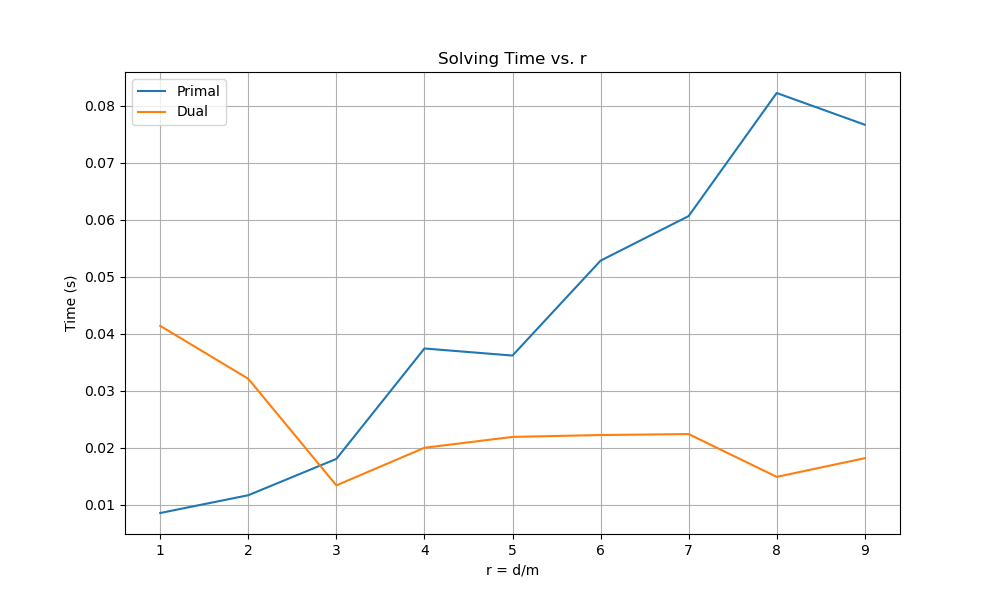
\includegraphics[width=1\linewidth]{Primal-dual Problem solving time from 1 to 10.png}
            \caption{Primal-dual Problem solving time from 1 to 10}
        \end{figure}
        
        简述题:\\
        这个r的比值我从1取值到了10,可以看到,特征维度和样例数量的比值较低的时候,primal问题明显消耗时间少一些,所以此时r小,更适合解决原问题。而当r的值上去了之后
        我们可以发现,primal 问题的解决时间明显慢下来了,所以此时适合解决对偶问题。
    \end{enumerate}
\end{solution}

\newpage

\section{[15pts] Kernel Function in Practice}

\texttt{lab3/svm\_kernel.py}中构造了异或(XOR)问题, 如图~\ref{xor}~所示. 该问题是线性不可分的.
\begin{figure}[h]
    \centering
    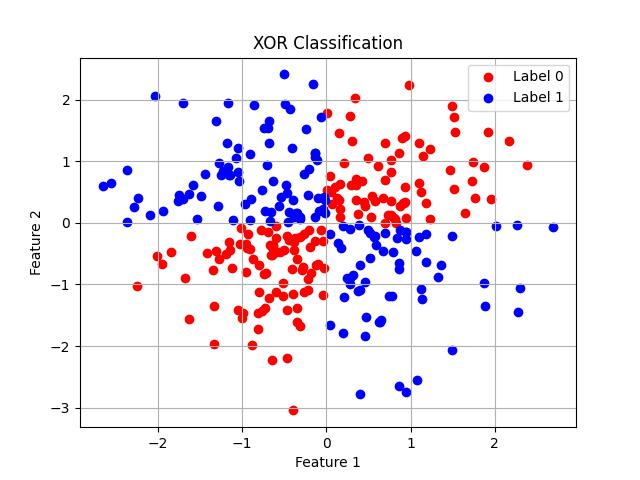
\includegraphics[width=0.5\textwidth]{lab3/XOR_data.jpg}
    \caption{异或(XOR)问题}
    \label{xor}
\end{figure}

本题中我们将通过实验了解核函数的选择对于SVM解决非线性问题的影响. 请使用\href{https://scikit-learn.org/stable/modules/generated/sklearn.svm.SVC.html}{ sklearn包中的SVM分类器}完成下述实验: 
\begin{enumerate}
    \item[(1)] \textbf{[6pts]} 请分别训练线性核SVM分类器和高斯核(RBF核) SVM分类器, 并绘制出各自的决策边界.
    \item[(2)] \textbf{[6pts]} sklearn还允许自定义核函数, 参考\texttt{lab3/svm\_kernel\_custom.py}的用法, 编写核函数$\kappa(\vx, \vx') = \frac{1}{1+\|\vx-\vx'\|_2^{2}}$, 训练该核函数的SVM分类器, 并绘制出决策边界. 
\end{enumerate} 
具体的实验要求可以参考\texttt{lab3/svm\_kernel.py}的\texttt{main}部分. 请将\texttt{lab3/svm\_kernel\_solution.py}中的代码和三个核函数分别对应的决策边界图提交至下方的解答处. 
\vspace{5pt}

最后, 请直接回答 \textbf{[3pts]}:三个核函数, 各自能够解决异或(XOR)分类问题吗?

\begin{solution}
    此处用于写解答(中英文均可)
    
    求解代码为:
    \lstinputlisting[language=Python]{lab3/svm_kernel_solution.py}
    
    决策边界为:
    \begin{figure}[h]
        \centering
        \begin{subfigure}[b]{0.3\textwidth}
            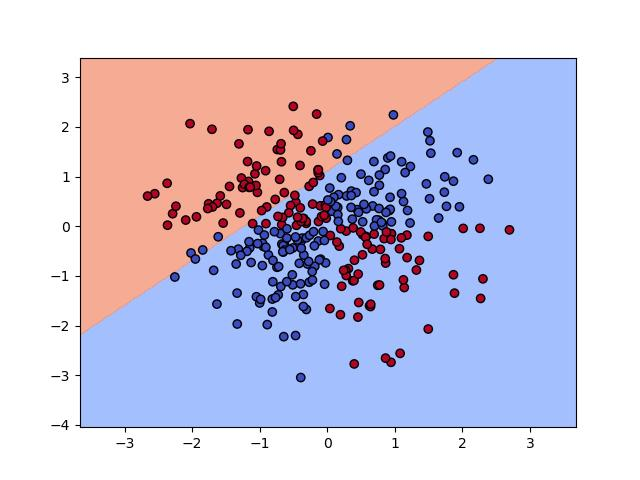
\includegraphics[width=\textwidth]{clf_linear.jpg}
            \caption{clf\_linear}
        \end{subfigure}
        \begin{subfigure}[b]{0.3\textwidth}
            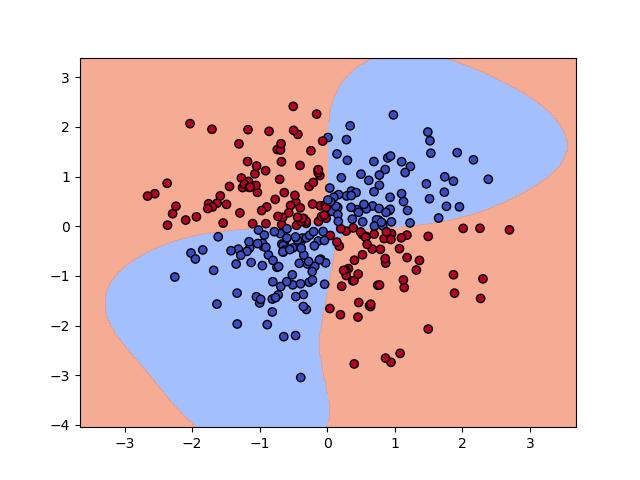
\includegraphics[width=\textwidth]{clf_rbf.jpg}
            \caption{clf\_rbf}
        \end{subfigure}
        \begin{subfigure}[b]{0.3\textwidth}
            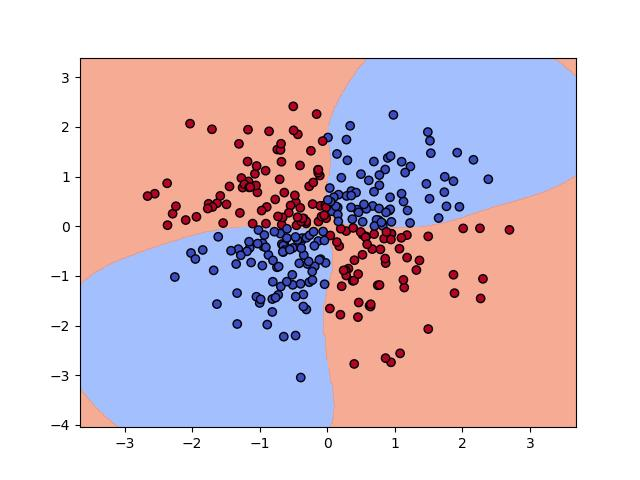
\includegraphics[width=\textwidth]{clf_custom.jpg}
            \caption{clf\_custom}
        \end{subfigure}
    \end{figure}
        
    能否解决异或(XOR)分类问题:明显第一个效果不好,后面两个可以解决xor问题。
\end{solution}

\newpage

\section{[30pts] Maximum Likelihood Estimation}
给定由$m$个样本组成的训练集$D=\left\{(\vx_1,y_1),(\vx_2,y_2),\cdots,(\vx_m,y_m)\right\}$, 其中$\vx_i\in\mathbb{R}^{d}$是第$i$个示例, $y_i\in\mathbb{R}$是对应的实值标记. 令$\mX\in\mathbb{R}^{m\times d}$表示整个训练集中所有样本特征构成的矩阵, 并令$\vy\in\mathbb{R}^{m}$表示训练集中所有样本标记构成的向量. 线性回归的目标是寻找一个参数向量$\vw\in\mathbb{R}^{d}$, 使得在训练集上模型预测的结果和真实标记之间的差距最小. 对于一个样本$\vx$, 线性回归给出的预测为$\hat{y}=\vw^\top\vx$,\footnote{本题不考虑偏移$b$, 可参考教材第3章将偏移$b$吸收进$\vw$. } 它与真实标记$y$之间的差距可以用平方损失$(\hat{y}-y)^2$来描述. 因此, 在整个训练集上最小化损失函数的过程可以写作如下的优化问题:
\begin{equation}
    \vw^\star=\underset{\vw}{\arg\min}\|\mX\vw-\vy\|_2^2
    \label{linear_regression_target}
\end{equation}
\begin{enumerate}
    \item[(1)] \textbf{[8pts]} 考虑这样一种概率观点: 样本$\vx$的标记$y$是从一个高斯分布$\mathcal{N}(\vw^\top\vx,\sigma^2)$中采样得到的. 这个高斯分布的均值由样本特征$\vx$和模型参数$\vw$共同决定, 而方差是一个额外的参数$\sigma^2$. 基于这种概率观点, 我们可以基于观测数据对高斯分布中的参数$\vw$做极大似然估计. 请证明: $\vw$的极大似然估计结果$\vw_{\mathrm{MLE}}$与式~\eqref{linear_regression_target}~中的$\vw^\star$相等;
	
    \item[(2)] \textbf{[9pts]} 极大似然估计容易过拟合, 一种常见的解决办法是采用最大后验估计: 沿着上一小问的思路, 现在我们希望在概率建模下对参数$\vw$做最大后验估计. 为此, 引入参数$\vw$上的先验$p(\vw)=\mathcal{N}(\vzero,\lambda\mat{I})$. 其中, 均值$\vzero$是$d$维的全$0$向量, $\mI$是$d$维单位矩阵, $\lambda>0$是一个控制方差的超参数. 现在, 请推导对$\vw$做最大后验估计的目标函数, 并讨论一下该结果与``带有$\mathrm{L}_2$范数正则项的线性回归"之间的关系;
	
    \item[(3)] \textbf{[9pts]} 沿着上一小问的思路, 我们尝试给参数$\vw$施加一个拉普拉斯先验. 简便起见, 我们假设参数$\vw$的$d$个维度之间是独立的, 且每一维都服从$0$均值的一元拉普拉斯分布, 即:
    \begin{equation}
	\begin{aligned}
	& p(\vw)=\prod_{j=1}^{d}p(w_j)\;, \\
	& p(w_j)=\mathrm{Lap}(w_j\mid 0,\lambda),\;j=1,2,\ldots,d\;.
	\end{aligned}
    \end{equation}
    请推导对$\vw$做最大后验估计的目标函数, 并讨论一下该结果与``带有$\mathrm{L}_1$范数正则项的线性回归"之间的关系;

    \textit{Note: 由参数$\mu$, $\lambda$确定的一元拉普拉斯分布的概率密度函数为:}
    \begin{equation}
	\mathrm{Lap}(w\mid\mu,\lambda)=\frac{1}{2\lambda}\exp\left(-\frac{|w-\mu|}{\lambda}\right)\;.
    \end{equation}	
    \item[(4)] \textbf{[4pts]} 基于(2)和(3)的结果, 从概率角度讨论为什么$\mathrm{L}_{1}$范数能使模型参数更稀疏.
\end{enumerate}
\begin{solution}
(1)我们对这个做一个guass分布:\\
\[  f(x) = \frac{1}{\sqrt{2\pi}\sigma}exp(-\frac{(x- \mu)^2}{2\sigma^2})\]
带入这个guass分布$N(\vw^{\top}\vx, \sigma^2)$,所以可以得到极大似然函数如下:\\
\[  L(\vw) = \prod_{i=1}^{d}\frac{1}{\sqrt{2\pi}\sigma} exp(-\frac{(y_i - \vw^{\top}x_i)^2}{2\sigma^2})\]
做对数极大似然:\\
\[  \log L(\vw) = -\frac{m}{2}\log(2\pi \sigma^2) - \frac{1}{2\sigma^2}\sum_{i=1}^{m}(y_i - \vw^{\top}x_i)\]
由于第一个项是个无关项,然后我们可以得到这个式子的最小化的形式:\\
\[  \vw{MLE} = \underset{\vw}{\arg\min}\{\frac{1}{2\sigma^2}\sum_{i=1}^{m}(y_i - \vw^{\top}x_i)\}\]
\[ =\underset{\vw}{\arg\min}\|\mX\vw-\vy\|_2^2\]
所以可以得到这个式子于式子4.1中的$\vw^\star$ 相等.\\

(2)首先由于要做最大后验分布,可以有贝叶斯公式得到:\\
\[  p(\vw|X, y) \propto p(y|X,\vw) p(\vw)\]
我们可以针对这个做最大后验,取一个负对数函数:\\
\[  \underset{\vw}{\arg\min} \log p(\vw|X, y) \propto -\log p(y|X,\vw) -\log p(\vw)\]
所以我们可以得到,由这个第一问知道,我们的$p(y|X,w)$是很容易求出来的,这个等价于$\frac{1}{2\sigma^2}\|\mX\vw-\vy\|_2^2$,所以我们只需要计算$p(w)$即可,由于这个东西符合多维guass分布,所以可以得到:\\
\[  p(\vw) = \frac{1}{(2\pi \lambda)^{d/2}}exp(-\frac{1}{2\lambda}\|\vw\|^2 )\]
\[  -\log p(\vw) = \frac{1}{2\lambda}\|\vw\|^2 + \frac{d}{2}\log(2\pi \lambda) \propto \frac{1}{2\lambda}\|\vw\|^2 \]
所以综上我们可以得到这个:\\
\[  \underset{\vw}{\arg\min} \log p(\vw|X, y) \propto \frac{1}{2\sigma^2}\|\mX\vw-\vy\|_2^2 +\frac{1}{2\lambda}\|\vw\|^2 \]
这个形式是等价于$L_2$正则化项的,由$L_2$正则化项的标准表达可以得到:\\
\[  L_2 = L_{data} + \sigma \|\vw\|_2^2\]
所以这个结果跟正则化这个是等价的,可以得到$\sigma = \frac{1}{2\lambda}$.说明在这种先验函数的前提下,这个式子符合一种``带有$\mathrm{L}_2$范数正则项的线性回归"之间的关系。

(3)对于这个题的laplace先验,我们只需要对$p(\vw)$进行重新计算即可,整个方法同上,我们仍然取负对数:\\
\[  \underset{\vw}{\arg\min} \log p(\vw|X, y) \propto -\log p(y|X,\vw) -\log p(\vw)\]
对于$p(\vw)$\\
\[  p(\vw) = \prod_{j=1}^{d} \frac{1}{2\lambda}exp(-\frac{|w_j|}{\lambda})\]
\[  p(\vw) \propto \sum_{i=1}^{d}\frac{|w_j|}{\lambda}\]
所以我们可以得到这个结果:\\
\[  \underset{\vw}{\arg\min} \log p(\vw|X, y) \propto \frac{1}{2\sigma^2}\|\mX\vw-\vy\|_2^2 + \sum_{i=1}^{d}\frac{|w_j|}{\lambda} \]
这个形式是等价于$L_1$正则化项的,由$L_1$正则化项的标准表达可以得到:\\
\[  L_1 = L_{data} + \sigma \|\vw\|_1\]
所以这里的$\sigma = \frac{1}{\lambda}$

(4).模型的参数的稀疏程度跟所选取的函数有密切关系,拉普拉斯先验分布的特点是它在零点处有一个尖峰,并且随着远离零点,概率密度迅速下降。这意味着在贝叶斯推断中,模型更倾向于选择接近零的参数值,因为这些值在先验分布中具有更高的概率。当我们在后验分布中最大化时,这种先验的偏好会导致许多参数的估计值趋向于零,从而产生稀疏解\\
而且,L1 正则化在参数空间中引入了非平滑的约束,这导致目标函数在参数空间中形成“尖角”,即在某些方向上,即使是很小的移动也会导致正则化项的显著增加。这些“尖角”恰好对应于参数为零的点,因此在优化过程中,解往往会“卡”在这些尖角上,使得相应的参数为零。
这就是为什么$\mathrm{L}_{1}$范数能使模型参数更稀疏.
\end{solution}

\newpage
\section*{Acknowledgments}
允许与其他同样未完成作业的同学讨论作业的内容, 但需在此注明并加以致谢; 如在作业过程中, 参考了互联网上的资料 (包括生成式模型的结果), 且对完成作业有帮助的, 亦需注明并致谢.

\end{document}
